% Appendix %%%%%%%%%%%%%%%%%%%%%%%%%%%%%%%%%%%%%%%%%%%%%%%%%%%%%%%
\begin{appendices} \appendixpage \noappendicestocpagenum \addappheadtotoc
{}
\chapter{Computing Coursework Assessment Criteria} \label{chap:Appendices}

Here is the marking scheme I will use:

	\begin{enumerate}
    \item You would get 100 pts if,
			\begin{enumerate}
				\item All the in-class scripts\footnote{{\it in-class scripts} are the ones that were give to you to practice with, which you only had to reproduce without error, while {\it assigned practicals / problems} are the assignments/problems you have been given that involve the writing of new scripts or the modification of existing ones. } were in place (in the code 
				directory in the respective week's directory) and functional 
				when run on my computer
        \item All the assigned practicals / problems are complete and functional, 
        and give the right answers
        \item The scripts are all up to the the mark in terms of internal documentation and commenting
        \item There is a neat {\tt readme} file detailing all the 
        scripts and what they do week 1 onwards.
      \end{enumerate}

    \item For every in-class script that gives a syntax error, 5 pts deducted, and for every script that gives an error because of wrong path (e.g., absolute) assignment, 2 pts deducted.
    \item For every missing script or assigned practical/problem, 10 pts deducted
    \item For every assigned practical/problem, 5 pts deducted for 
    wrong answer if applicable (that is, script runs without error, but 
    gives wrong numerical or text output).
    \item For every missing {\tt readme} file, 1 pt deducted.
		\item For every extra, non-script file in {\tt Code} directory, 0.5 
		pt deducted.
		\item For every {\it valid} script file in {\tt Code} directory 
		lacking an appropriate extension, 0.5 pt deducted.
		\item For every result of a code/script run not saved to a separate 
		{\tt Results} directory, 1 pt deducted.
    \item For every extra-credit question completed, 2.5 pts added.
	\end{enumerate}

From the points left after implementing the above criteria, I will 
exercise my judgement to deduct furtjer marks if the weekly directory 
structure is disorganized, the code inadequately commented or 
insufficiently documented, or the written components of practicals are 
not up to the mark. 

You will get feedback if these issues needed to be addressed in the 
final written assessment. The final marks will be based upon these 
weekly points and a coursework marking criteria (See below). I will 
 up- or down-weigh the contribution of each week to the 
overall marks based upon the difficulty level. 

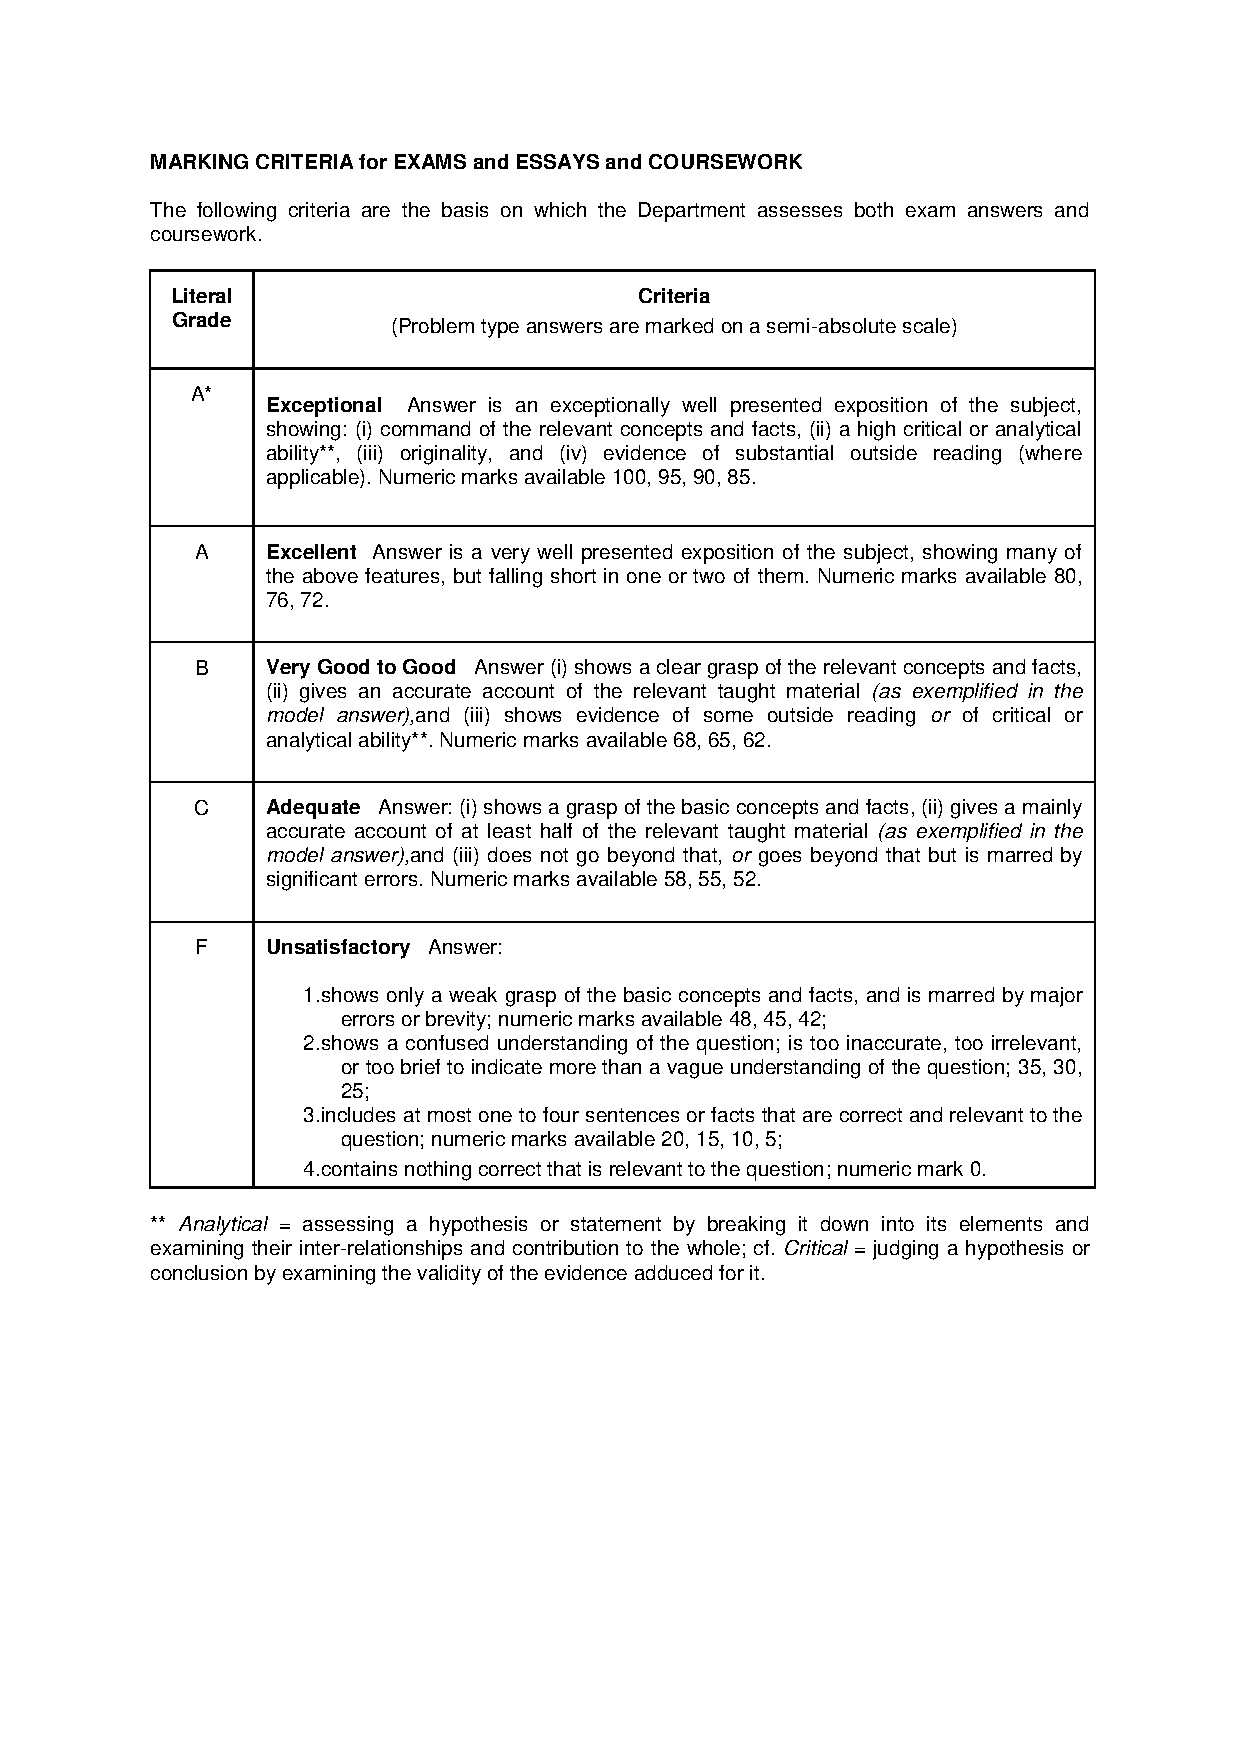
\includepdf[pagecommand={}]{MARKING_CRITERIA.pdf}
\end{appendices}
